\pagestyle{main}
\begin{multicols}{2}
\noindentсвободные члены в равенстве\newline
\textsl{P(x) = (b - c) $x^2$ + (c - a)x + (a - b) = (b - c)(x - 1)(x - 1234)} , получаем \textsl{a - b = 1234(b - c)} , откуда \textsl{a = 1235b - 1234b}. Тогда значение первого трехчлена в точае 1 равно \textsl{a + b + c = 1236b - 1233c = 3(412b - 411c)}, т.е делится на 3; значит, оно не может равняться 2009.\\
8. $50\sqrt{2}$\\
\noindentПронумеруем в квадрате строки (снизу вверх) и столбцы (слева направо) числами от 1 до 100; будем обозначать клетку парой номеров ее строки и столбца. Назовем \textsl{расстоянием} между клетками расстояние между их центрами. Клетки назовем \textsl{парными}, если числа в них различаются на 5000. Заметим, что расстояние от клетки (50, 50) до любой другой (в частности, до парной ей) не превосходит $\sqrt{50^2 + 50^2}$ =
\vspace{-0,5\baselineskip}
\begin{multicols}{2}
\begin{minipage}{\linewidth}
\centering
\resizebox{\linewidth}{!}{
\begin{tabular}{|c|c|c|c|c|c|c|c|}
    \hline
     64&57&56&49&48&47&46&45\\
     \hline
     63&58&55&50&41&42&43&44\\
     \hline
     62&59&54&51&40&39&38&37\\
     \hline
     61&60&53&52&33&34&35&36\\
     \hline
     4&5&12&13&32&31&30&29\\
     \hline
     3&6&11&14&25&26&27&28\\
     \hline
     2&7&10&15&24&23&22&21\\
     \hline
     1&8&9&16&17&18&19&20\\
     \hline
\end{tabular}
}
\end{minipage}

\vfill\null
\columnbreak

\begin{adjustwidth}{0,2cm}{}
= $50\sqrt{2}$. Значит, и минимальное расстояние между парными клетками также не превосходит $50\sqrt{2}$. На рисунке 10 приведен пример расстановки чисел 1, ..., 64
\end{adjustwidth}
\end{multicols}
\vspace{-0,5\baselineskip}
\noindentв квадрате 8x8, при которойминимальное расстояние между центрами парных клеток (в данном примере числа в парных клетках отличаются на 32) достигает своего наибольшего значения $4\sqrt{2}$\\
\noindentЭтот пример легко обобщить, чтобы расставить нужным образом числа в квадрате 100x100.

\small\begin{center}
    \noindent\fontsize{8}{9}\textbf{РЕГИОНАЛЬНЫЙ ЭТАП XLIV ВСЕРОССИЙСКОЙ\\
    ОЛИМПИАДЫ ШКОЛЬНИКОВ ПО ФИЗИКЕ}\\
    \textsl{7 класс}
\end{center}
1. L = $v_0$t = 2,5км/ч . 2ч = 5км.\quad\quad\quad2. V = 20мл\\

\noindent3. $\Delta$L = $L_B$ - $L_A$ = $\frac{L}{2}$($\frac{v_2 - v_1}{v_2 + v_1}$) = 0,18 мили.\\

\noindent4. d = 0,5 мм, h = 0,1 мм.
\begin{center}
    \textsl{8 класс}
\end{center}
\noindent1. Безразлично, куда бежать вначале: вверх или вниз.\\
\noindent2. $\Delta$$t_3$ = 1,25$^\circ$C.\quad\quad3. M = 12,5 г, L = 41,5 мм.\\
\noindent4. m = $\frac{\rho_0abc^2}{c - b}$ = 2 кг.
\begin{center}
    \textsl{9 класс}
\end{center}
\noindent1. t = 20 мин.\quad2. $m_2$ = $m_1$$\frac{c_1}{2c_2}$$\frac{\alpha(t_1^2 - t_0^2) + 2(t_1 - t_0)}{t_0 - t_2}$ $\approx 0,707$ кг.
\begin{multicols}{2}
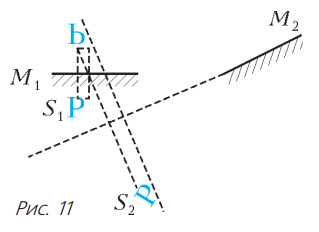
\includegraphics[width=\linewidth]{Pic1.png}
\vfill\null
\columnbreak
\noindent\textbf{3.} Все три резистора соединены параллельно и подключены к полюсам батарейки; U = 3 B: $I_2 - I_1$ = 2 мА.\\
\noindent\textbf{4.} \textsl{$N_1$} = $\sqrt{50}$ $N_0$ $\approx$170 кадров/с.\\

\noindent\textbf{5.} В системе есть всего два изображения, полученные в зеркалах \textsl{$M_1$} и \textsl{$M_2$} (рис.11).
\end{multicols}
\begin{center}
\textsl{10 класс}
\end{center}

\noindent\textbf{1.} $\textsl{v}_\text{max} = \sqrt{\frac{\mu\textsl{g}L}{2}(1 + \frac{m}{M})}$.\quad\quad\textbf{2.} F = 0,65 \textsl{mg}.\\

\noindent\textbf{3.} При \textsl{$T_1$} = $\frac{1}{4}$\textsl{$T_0$} и \textsl{$T_2$} = $\frac{3}{4}$\textsl{$T_0$}.\quad\quad\textbf{4.} \textsl{$R_\text{AB}$} = $\frac{5\textsl{R}}{48}$ = 10 Ом.\\

\noindent\textbf{5.} $\textsl{V}_0 \approx (0.82 \pm 0.05)\ \text{л}.$
\columnbreak
\begin{center}
    \textsl{11 класс}
\end{center}
\noindent\textbf{1.} \textsl{$K_2$} = 2,25 \textsl{П} = 2,25 Дж.\\
\noindent\textbf{2.} $\textsl{H} = \frac{\textsl{g}\tau_1^2}{2} = 5 \text{м}; \mu = \frac{\textsl{M}}{2\tau_2} = 0.2 \text{кг/с}.$\quad\textbf{3.} $\textsl{Q} = \frac{\textsl{C}\mathcal{E}^2}{8}\left(\frac{R}{R + r}\right)^2$.\\
\noindent\textbf{4.} tg$\phi_1 \approx 0,347 , \phi_1 \approx 19,1^\circ$.\\
\noindent\textbf{5.} Тепло подводится на всех верхних горизонтальных и на всех левых вертикальных участках, \textsl{Q} = 9,18\textsl{$p_0V_0$}.
\begin{center}
    \textbf{ВСЕРОССИЙСКАЯ СТУДЕНЧЕСКАЯ ОЛИМПИАДА}\\
    \textbf{ПО ФИЗИКЕ}
\end{center}
\noindent\textbf{1.} $\textsl{s}_1 = \frac{2\textsl{L}}{\sqrt{5}}, \textsl{s}_2 = \frac{\textsl{L}}{\sqrt{5}}.$\quad\quad\quad\textbf{2.} $\textsl{T} = \frac{2\pi\textsl{L}}{\sqrt{12\textsl{g}\textsl{R}}}$.\\
\noindent\textbf{3.} $\omega_1 = \frac{\Omega}{3},\omega_2 = \frac{2\Omega}{3},\textsl{v}_1 = \textsl{v}_2 = \sqrt{\frac{\textsl{v}^2}{4} + \frac{\Omega^2R^2}{36}}$.\\
\noindent\textbf{4.} $\frac{1}{16}\frac{\left\lvert \vec{\textsl{r}}_{12} \times (\vec{\textsl{v}}_2 - \vec{\textsl{v}}_1) \right\rvert^2}{\textsl{R}^2}<\frac{(\vec{v_2} - \vec{v_1})^2}{4} + \textsl{Gm}(\frac{1}{2\textsl{R}} - \frac{1}{\textsl{r}})$.\\
\noindent\textbf{5.} Если $\frac{\textsl{H}}{2}\leq \textsl{h}_{max}$,то $\textsl{D}_{max} = 2\textsl{r} + (\textsl{n} - 1)\frac{\textsl{r}\rho\textsl{g}\textsl{H}^2}{4\sigma}$, если $\frac{\textsl{H}}{2} > \textsl{h}_{max}$, то $\textsl{D}_{max} = 2\textsl{r} + 4(\textsl{n} - 1)(\textsl{H} - \textsl{h}_{max})\frac{\textsl{r}}{\textsl{d}}$, где $\textsl{h}_{max} = \frac{\textsl{4}\sigma}{\rho\textsl{gd}}$ - максимальная высота столба жидкости в капилляре.\\
\noindent\textbf{6.} $\textsl{T}_2$ = $\frac{5}{3}\textsl{T}$.\quad\textbf{7.} \textsl{F} = $\frac{\textsl{p}_m\textsl{B}}{\textsl{R}}$.\quad\textbf{8.} \textsl{W} = $\frac{1}{2}(\frac{\textsl{q}^2}{2\pi\epsilon_0\textsl{R}} - \textsl{q}\phi)$.\quad\textbf{9.} \textsl{I} = $\frac{\textsl{I}_0}{4}$.\\

\begin{center}
\begin{tabular}{|c|}
\hline

\includegraphics[width=\linewidth]{Pic2.png} \\
\hline
\\
\textbf{НОМЕР ПОДГОТОВИЛИ}\\
\textbf{С.А.Дориченко, А.А.Егоров, Е.М.Епифанов,}\\
\textbf{С.П.Коновалов, А.Ю.Котова, В.А.Тихомирова,}\\
\textbf{А.И.Черноуцан}\\
\textbf{НОМЕР ОФОРМИЛИ}\\
\textbf{А.Ващенко, Д.Н.Гришукова, А.Е.Пацхверия,}\\
\textbf{М.В.Сумнина}\\
\textbf{ХУДОЖЕСТВЕННЫЙ РЕДАКТОР}\\
\textbf{Е.В.Морозова}\\
\textbf{КОМПЬЮТЕРНАЯ ГРУППА}\\
\textbf{Е.А.Митченко, Л.В.Калиничева}\\
\hline
\\
\textbf{Журнал «Квант» зарегистрирован в Комитете РФ}\\
\textbf{по печати. Рег. св-во №0110473}\\
\\
\textbf{Адрес редакции:}\\
\textbf{119296 Москва, Ленинский проспект, 64-А, «Квант»}\\
\textbf{Тел.: 930-56-48}\\
\textbf{Е-mail: admin@kvant.info, math@kvant.info,}\\
\textbf{phys@kvant.info}\\
\textbf{Сайт: kvant.info}\\
\hline
\\
\textbf{Отпечатано в ОАО ордена Трудового Красного Знамени}\\
\textbf{«Чеховский полиграфический комбинат»}\\
\textbf{142300 г.Чехов Московской области,}\\
\textbf{Сайт: www.chpk.ru E-mail: marketing@chpk.ru}\\
\textbf{Факс: 8(49672) 6-25-36, факс: 8(499) 270-73-00}\\
\textbf{Отдел продаж услуг многоканальный: 8(499) 270-73-59}\\
\hline
\end{tabular}
\end{center}
\end{multicols}
\newpage